\section{Imitation Dynamics}
Η δεύτερη εξελικτική δυναμική που θα παρουσιαστεί είναι αυτή των Imitation Dynamics - δυναμική μίμησης. Στην περίπτωση αυτή, δεν υπολογίζεται η νέα κατανομή του πληθυσμού αυστηρά ως συνάρτηση του fitness της κάθε στρατηγικής για κάθε γενιά, αλλά υιοθετείται μία πιο απλή και ίσως πιο εφαρμόσιμη στην πραγματικότητα λογική: σε κάθε γενιά, βρίσκουμε τη στρατηγική (ή σε περίπτωση ισοπαλίας τις στρατηγικές) που ανταποκρίθηκαν καλύτερα. Έπειτα, έχοντας ορίσει τον αριθμό K των παικτών που αλλάζουν στρατηγική ανά γενιά, επιλέγονται τυχαία K παίκτες μη βέλτιστης στρατηγικής και υιοθετούν μία εκ των βέλτιστων στρατηγικών, πάλι τυχαία, σε περίπτωση ισοβαθμίας. 

Να επισημανθεί ότι η επιλογή γίνεται μόνο μεταξύ παικτών μη βέλτιστης στρατηγικής και όχι μεταξύ όλων των παικτών του πληθυσμού. Αυτό θεωρούμε πως ανταποκρίνεται περισσότερο στην πραγματικότητα - αν βρίσκεται κάποιος παίκτης ήδη στη βέλτιστη στρατηγική, γιατί να σκεφτεί να αλλάξει στρατηγική; Η επιλογή αυτή έχει μερικές συνέπειες στα αποτελέσματα που παρουσιάζονται παρακάτω.

Για την εύρεση της βέλτιστης στρατηγικής χρησιμοποιείται υπολογισμός του score παρόμοιος με αυτόν της περίπτωσης των fitness dynamics, ώστε να εξοικονομείται χρόνος κατά την εκτέλεση τως προγραμμάτων. Δηλαδή, δεν προσομοιώνονται πραγματικά τα matches μεταξύ κάθε παίκτη, αλλά υπολογίζονται τα scores με βάση τις απολαβές κάθε στρατηγικής εναντίον κάθε στρατηγικής και τους αντίστοιχους πληθυσμούς.

Όπως θα παρουσιαστεί παρακάτω, κατά τη θεωρητική παρουσίαση της συνάρτησης TourTheImi, η διαδικασία αυτή μπορεί να διατυπωθεί με τη βοήθεια μαρκοβιανής αλυσίδας, όπου καταστάσεις είναι οι διάφορες πιθανές κατανομές πληθυσμού, με βάση το άθροισμα των αρχικών πληθυσμών (τον συνολικό πληθυσμό) και τον αριθμό στρατηγικών που εμπλέκονται στη διαδικασία. Στην αναφορά του κ. Κεχαγιά βρίσκεται το θεωρητικό υπόβαθρο αυτών που θα συζητηθούν αργότερα: θεωρούμε αρχικά την r-state μαρκοβιανή αλυσίδα, όπου κάθε κατάσταση είναι η στρατηγική του κάθε παίκτη ξεχωριστά, π.χ. για N = 5 παίκτες και 3 στρατηγικές, πιθανό r-state είναι το (11323). Θεωρούμε έπειτα, τις s-states, όπου κατάσταση είναι ο πληθυσμός της κάθε στρατηγικής, στο προηγούμενο παράδειγμα το s-state θα ήταν (212). Ουσιαστικά πρόκειται για grouping διάφορων r-states σε ένα s-state, το οποίο, λόγω του ότι δε μας ενδιαφέρει πραγματικά ο κάθε παίκτης ξεχωριστά, αλλά ο συνολικός πληθυσμός της κάθε στρατηγικής, είναι ισοδύναμο. Αποδεικνύεται ότι η διαδικασία r(t) είναι lumpable και άρα ότι η s(t) είναι μαρκοβιανή αλυσίδα. Η θεωρητική αυτή γνώση είναι απαραίτητη για την υλοποίηση της TourTheImi παρακάτω.
\subsection{Η συνάρτηση TourSimImi}
Υλοποιείται, αρχικά, συνάρτηση προσομοίωσης του εξελικτικού πρωταθλήματος με δυναμική μίμησης [POP, BST]\- =\- TourSimImi\- (B,\- Strategies,\- POP0,\- K,\- T, \-J, \- mode). Οι είσοδοι και έξοδοι της συνάρτησης είναι όμοιες με αυτές της TourSimFit, με έξτρα όρισμα μία ακέραια τιμή K που προσδιορίζει τον αριθμό παικτών που αλλάζουν στρατηγική ανά γενιά. Το έξτρα όρισμα mode (η συνάρτηση τρέχει με default τιμή "Individual") λαμβάνει τιμές "Individual" και "Total" και αναφέρεται στον τρόπο με τον οποίο επιλέγεται η βέλτιστη στρατηγική: στην περίπτωση "Individual", επιστρέφεται απλά η στρατηγική του καλύτερου παίκτη, ενώ στην περίπτωση "Total" επιστρέφεται η στρατηγική με το μεγαλύτερο άθροισμα scores ανά τους παίκτες που τη χρησιμοποιούν. Η επιλογή του mode επιφέρει σημαντικά διαφορετικά αποτελέσματα, όπως θα παρουσιαστεί παρακάτω.

Να σχολιαστεί επίσης ότι, σε περίπτωση που οι παίκτες με μη βέλτιστη στρατηγική είναι λιγότεροι από K, αλλάζουν στρατηγική όλοι οι παίκτες με μη βέλτιστη στρατηγική, σε πλήθος λιγότεροι από K. Παραδείγματος χάριν, βρισκόμαστε σε κατάσταση μόνο με All\_C και TitForTat, οι απολαβές με τη μέθοδο Individual είναι ίδιες και το $K = 1$. Υπάρχουν 0 άτομα με μη βέλτιστη στρατηγική, άρα δεν αλλάζει κανένας στρατηγική, μιας και $0<1$. Αντίστοιχα, αν οι μη βέλτιστοι παίκτες είναι 2 και το K είναι 3, θα αλλάξουν μόνο οι 2 και ούτω καθεξής.

\subsection{Η συνάρτηση TourTheImi}
Η συνάρτηση TourTheImi είναι το τελευταίο ζητούμενο της εργασίας. Έχει τη μορφή P\- =\- TourTheImi\- (B,\- Strategies,\- POP0,\- K,\- T,\- J,\- mode), με ορίσματα πλήρως πανομοιότυπα της συνάρτησης TourSimImi και έξοδο τον πίνακα μεταβάσεων της μαρκοβιανής αλυσίδας των s-states P. Στην πραγματικότητα, για τον υπολογισμό του πίνακα P, ο αρχικός πληθυσμός χρησιμοποιείται μόνο για να υπολογιστεί ο συνολικός πληθυσμός του πρωταθλήματος (άρα θα μπορούσε απλά να αντικατασταθεί από ένα όρισμα N) και ο αριθμός γενεών J δε χρησιμοποιείται καθόλου.

Για την ανάλυση αυτή θεωρούμε τα s-states του πρωταθλήματος ως τους αριθμούς των παικτών κάθε στρατηγικής, π.χ. για N = 9 έχουμε $s_1 = \begin{bmatrix} 0 & 0 & 9 \end{bmatrix}$, $s_2 = \begin{bmatrix} 0 & 1 & 8 \end{bmatrix}$ και ούτω καθεξής. Ανάλογα με το όρισμα mode, αναμένουμε ο πίνακας μετάβασης να έχει διαφορετική μορφή. Για παράδειγμα, στο mode Individual και με στρατηγικές All\_D, All\_C, και TitForTat, η κατάσταση $\begin{bmatrix} 0 & 5 & 4 \end{bmatrix}$ αναμένουμε να είναι absorbing, μιας και δεν υπάρχουν μη βέλτιστοι παίκτες και άρα να έχει μόνο μία μετάβαση, στον εαυτό της, με πιθανότητα 1. Αντίθετα, στην περίπτωση Total, η κατάσταση αυτή δε θα ήταν absorbing, καθώς η στρατηγική All\_C συγκεντρώνει περισσότερους συνολικούς πόντους.

Δημιουργείται και μία ακόμη συνάρτηση AnalyzeMarkovChain\- (P,\- POP0,\- Str\-at\-e\-gies,\- Title), η οποία είναι υπεύθυνη για την παραγωγή των διαγραμμάτων μετάβασης καταστάσεων που παρουσιάζονται παρακάτω. Η συνάρτηση αυτή, με βάση τον πίνακα P που υπολογίζεται από τη συνάρτηση TourTheImi και τον αρχικό πληθυσμό POP0, διαχωρίζει τις καταστάσεις σε μεταβατικές - transient, απορροφητικές - absorbing και την αρχική κατάσταση. Επίσης, κάνει την περαιτέρω διάκριση μεταξύ reachable και unreachable καταστάσεων με βάση την αρχική κατάσταση. Δημιουργεί διάγραμμα της κάθε κατάστασης, στο οποίο φαίνεται με χρώμα ο τύπος κατάστασης, φαίνονται οι πληθυσμοί της κάθε κατάστασης, τα ονόματα των στρατηγικών, που δίνονται με το όρισμα Strategies, και οι αντίστοιχες πιθανότητες μετάβασης πάνω από κάθε μετάβαση. Το όρισμα Title είναι ο τίτλος του διαγράμματος που προκύπτει. 
\subsection{Προσομοιώσεις}
Παρακάτω παρουσιάζονται κάποιες προσομοιώσεις οι οποίες παράγονται από τις συναρτήσεις που περιγράφηκαν παραπάνω και παρουσιάζουν ενδιαφέρον. Η κάθε προσομοίωση βρίσκεται στο αρχείο example.m σε κατάλληλο Section και με Run Section προκύπτουν ακριβώς τα αποτελέσματα που παρουσιάζονται παρακάτω.
\subsubsection{1η Προσομοίωση - Παράδειγμα χρήσης των Tour\-The\-Imi, Analyze\-Markov\-Chain και Tour\-Sim\-Imi}
Στην πρώτη προσομοίωση \ref{fig:TourTheImi153} παρουσιάζεται η μαρκοβιανή αλυσίδα που προκύπτει για τις στρατηγικές $\begin{bmatrix}All\_D&All\_C&TitForTat\end{bmatrix}$ σε μείγμα $\begin{bmatrix}1&5&3\end{bmatrix}$.
Από το διάγραμμα που προκύπτει παρατηρούμε ότι οι πιθανές απορροφητικές καταστάσεις είναι η $\begin{bmatrix}9&0&0\end{bmatrix}$, δηλαδή η επικράτηση της στρατηγικής $All\_D$, η $\begin{bmatrix}0&0&9\end{bmatrix}$, δηλαδή η επικράτηση της στρατηγικής $TitForTat$ και η $\begin{bmatrix}0&1&8\end{bmatrix}$, δηλαδή η επικράτηση της $TitForTat$ αλλά με επιβίωση της $All\_C$. Από τις πιθανότητες μετάβασης, που απεικονίζονται στα βέλη των μεταβάσεων, παρατηρούμε ότι η τελευταία απορροφητική κατάσταση έχει σημαντικά χαμηλότερη πιθανότητα να συμβεί σε σχέση με τις άλλες δύο. Ακόμη παρατηρούμε ότι οι καταστάσεις στις οποίες υπάρχουν μόνο οι συμπαθείς στρατηγικές ($All\_C$ και $TitForTat$), δηλαδή στρατηγικές οι οποίες ποτέ δεν λιποτακτούν πρώτες και άρα οι παίκτες των οποίων αποκτούν ίσα σκορ παίζοντας μεταξύ τους, μεταβαίνουν μόνο στον εαυτό τους καθώς δεν υπάρχουν παίκτες με σκορ χαμηλότερο του μεγίστου.

	\begin{figure}[h]
	      \centering
	      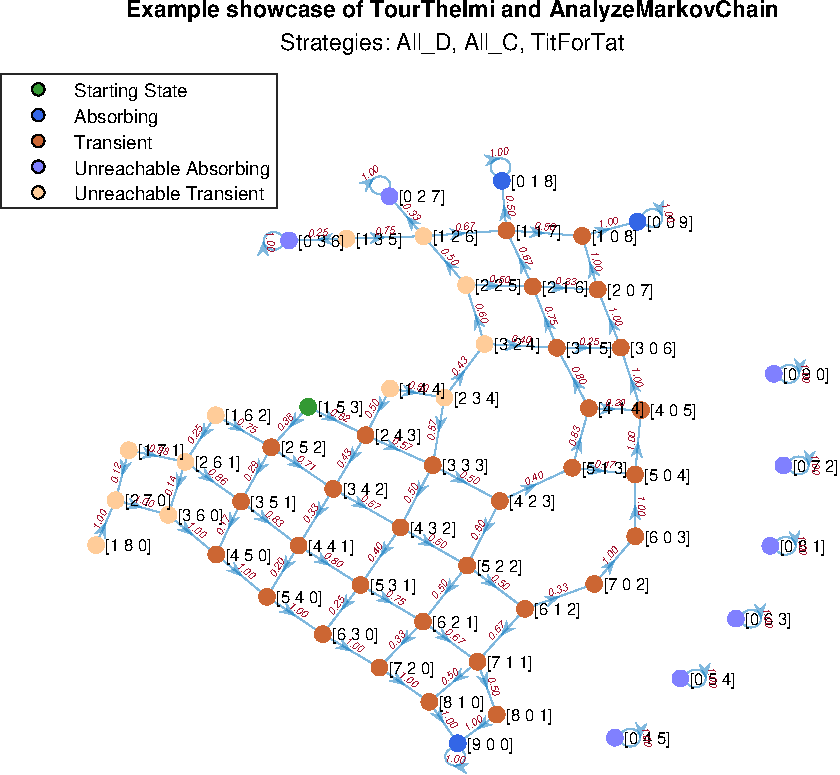
\includegraphics[width=0.95\textwidth]{Example showcase of TourTheImi and AnalyzeMarkovChain.pdf}
	      \caption{Example showcase of TourTheImi and AnalyzeMarkovChain}
	      \label{fig:TourTheImi153}
	\end{figure}
	
Στο Σχήμα \ref{fig:TourSimImi153} απεικονίζονται δύο εκτελέσεις της TourSimImi για το μείγμα στρατηγικών της παραπάνω προσομοίωσης. Παρατηρούμε ότι λόγω του τυχαίου τρόπου επιλογής των imitators, δηλαδή των παικτών που δεν έχουν την καλύτερη στρατηγική και αλλάζουν σε κάποια από τις καλύτερες, το τελικό μείγμα στρατηγικών είναι διαφορετικό για κάθε εκτέλεση του προγράμματος. Συγκεκριμένα στην (α) εκτέλεση παρατηρούμε $\begin{bmatrix}1&5&3\end{bmatrix} \rightarrow^* \begin{bmatrix}9&0&0\end{bmatrix}$ ενώ στην (β) εκτέλεση $\begin{bmatrix}1&5&3\end{bmatrix} \rightarrow^*	\begin{bmatrix}0&0&9\end{bmatrix}$, που όπως αναλύσαμε παραπάνω είναι πράγματι οι δύο πιο πιθανές απορροφητικές καταστάσεις.
	\begin{figure}[h]
		\centering
		\begin{subfigure}{.5\textwidth}
			\centering
	      	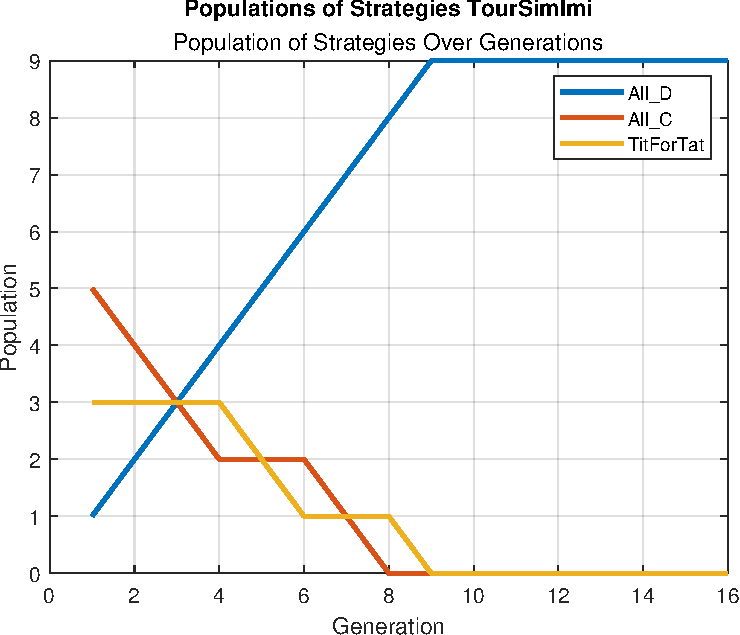
\includegraphics[width=.9\textwidth]{900.pdf}
			\caption{$\begin{bmatrix}9&0&0\end{bmatrix}$}
	      	\label{fig:900}
		\end{subfigure}%
		\begin{subfigure}{.5\textwidth}
			\centering
	      	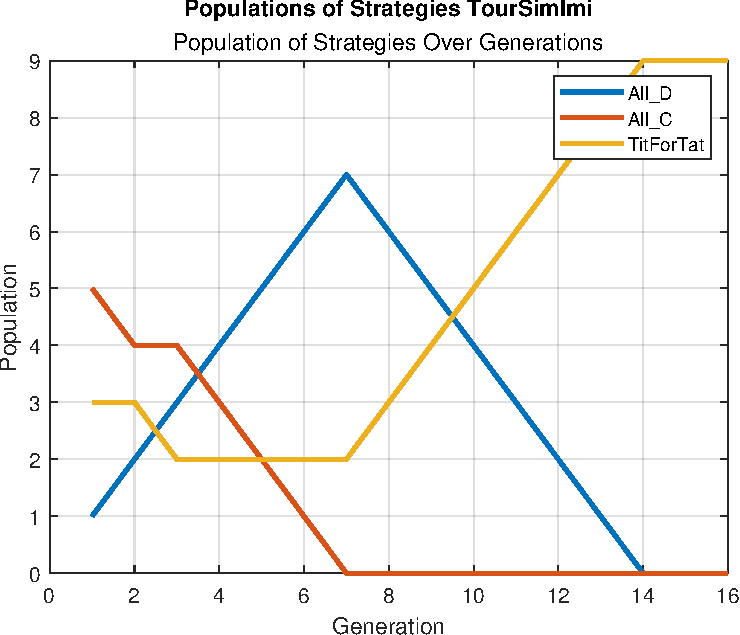
\includegraphics[width=0.90\textwidth]{009.pdf}
			\caption{$\begin{bmatrix}0&0&9\end{bmatrix}$}
	      	\label{fig:009}
		\end{subfigure}
		\caption{Absorbing States may differ even for the same Starting State}
		\label{fig:TourSimImi153}
	\end{figure}

\subsubsection{2η Προσομοίωση - Δοκιμή προεπιλεγμένης μεθόδου (Individual) για τον προσδιορισμό της καλύτερης στρατηγικής}
Στις δύο επόμενες προσομοιώσεις επιχειρείται να παρουσιαστεί η διαφορά στα αποτελέσματα που προκαλεί η διαφορετική μεθοδολογία επιλογής της καλύτερης στρατηγικής. Αρχικά (\ref{fig:TourTheImiIndividual}) παρουσιάζεται η μαρκοβιανή αλυσίδα που προκύπτει για αρχικό μείγμα στρατηγικών $\begin{bmatrix}1&4&5\end{bmatrix}$ και επιλογή μεθόδου ``Individual'', δηλαδή επιλογή της καλύτερης στατηγικής με σύγκριση των payoffs των στρατηγικών με παιχνίδια ένας εναντίον ενός για κάθε ζεύγος στρατηγικών.

Το αποτέλεσμα είναι αντίστοιχο αυτού της πρώτης προσομοίωσης \ref{fig:TourTheImi153}. Με λίγη παρατήρηση μπορούμε να οραματιστούμε μία νοητή καμπύλη μεταξύ των κορυφών των καταστάσεων $\begin{bmatrix}8&0&2\end{bmatrix}, \begin{bmatrix}6&1&3\end{bmatrix}, \begin{bmatrix}4&2&4\end{bmatrix}, \begin{bmatrix}2&3&5\end{bmatrix}$ η οποία χωρίζει τις λεκάνες απορροής των συμπαθών και των μη-συμπαθών στρατηγικών. Αν βρεθούμε σε κατάσταση κάτω από αυτή την καμπύλη θα καταλήξουμε στην απορροφητική κατάσταση επικράτησης της ``All\_D'', ενώ από κατάσταση πάνω από αυτή την καμπύλη θα καταλήξουμε σε μία από τις απορροφητικές καταστάσεις των συμπαθών στρατηγικών.
	\begin{figure}[h]
	      \centering
	      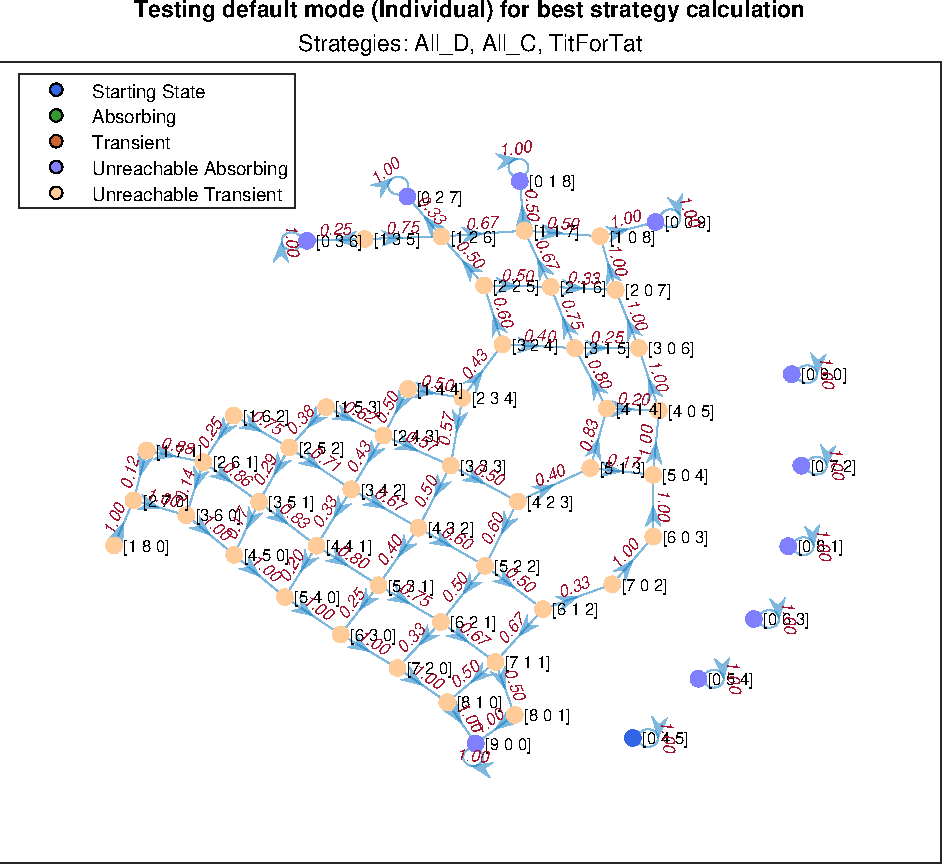
\includegraphics[width=0.95\textwidth]{Testing default mode (Individual) for best strategy calculation.pdf}
	      \caption{Testing default mode (``Individual'') for best strategy calculation with $POP0=\begin{bmatrix}1&4&5\end{bmatrix}$}
	      \label{fig:TourTheImiIndividual}
	\end{figure}
\subsubsection{3η Προσομοίωση - Δοκιμή μεθόδου ``Total'' για τον προσδιορισμό της καλύτερης στρατηγικής}
Στην τρίτη προσομοίωση (\ref{fig:TourTheImiTotal}) για ίδιο αρχικό μείγμα στρατηγικών $\begin{bmatrix}1&4&5\end{bmatrix}$ και επιλογή μεθόδου ``Total'', δηλαδή σύγκριση των payoffs των παικτών που προκύπτουν σε κάθε state από Axelrod με τους πληθυσμούς του state και επιλογή ως καλύτερη στρατηγική της στρατηγικής του παίκτη με το μεγαλύτερο συνολικό payoff.

Σε αντίθεση με την προηγούμενη προσομοίωση (\ref{fig:TourTheImiIndividual}) εδώ παρατηρούμε ότι το διάγραμμα είναι χωρισμένο σε τρεις ξεχωριστούς υπογράφους.
Ο πρώτος υπογράφος, αυτός που περιλαμβάνει την αρχική κατάσταση, είναι ο μόνος που περιλαμβάνει προσεγγίσιμη απορροφητική κατάσταση (την $\begin{bmatrix}0&0&10\end{bmatrix}$), η οποία είναι η επικράτηση της ``TitForTat''. Αυτό συμβαίνει διότι κατά την εύρεση της καλυτερης στρατηγικής στο mode ``Total'' οι συμπαθείς στρατηγικές συνεργάζονται μεταξύ τους και υπερνικούν λόγω του μεγαλύτερου πλήθους τους το προβάδισμα που δίνει η λιποταξία στην ``All\_D''
Ο δεύτερος υπογράφος είναι αυτός που περιλαμβάνει την απορροφητική κατάσταση που επικρατεί η ``All\_D'' ($\begin{bmatrix}10&0&0\end{bmatrix}$), η οποία όμως είναι μη προσπελάσιμη όπως και οι μεταβατικές καταστάσεις όλου του υπογράφου, για τον λόγο που περιγράφηκε παραπάνω.
Τέλος ο τρίτος υπογράφος είναι αυτός που περιλαμβάνει την απορροφητική κατάσταση που επικρατεί η ``All\_C'' ($\begin{bmatrix}0&10&0\end{bmatrix}$), η οποία είναι επίσης μη προσπελάσιμη όπως και οι μεταβατικές καταστάσεις όλου του υπογράφου, για τον λόγο που περιγράφηκε παραπάνω.

	\begin{figure}[h]
	      \centering
	      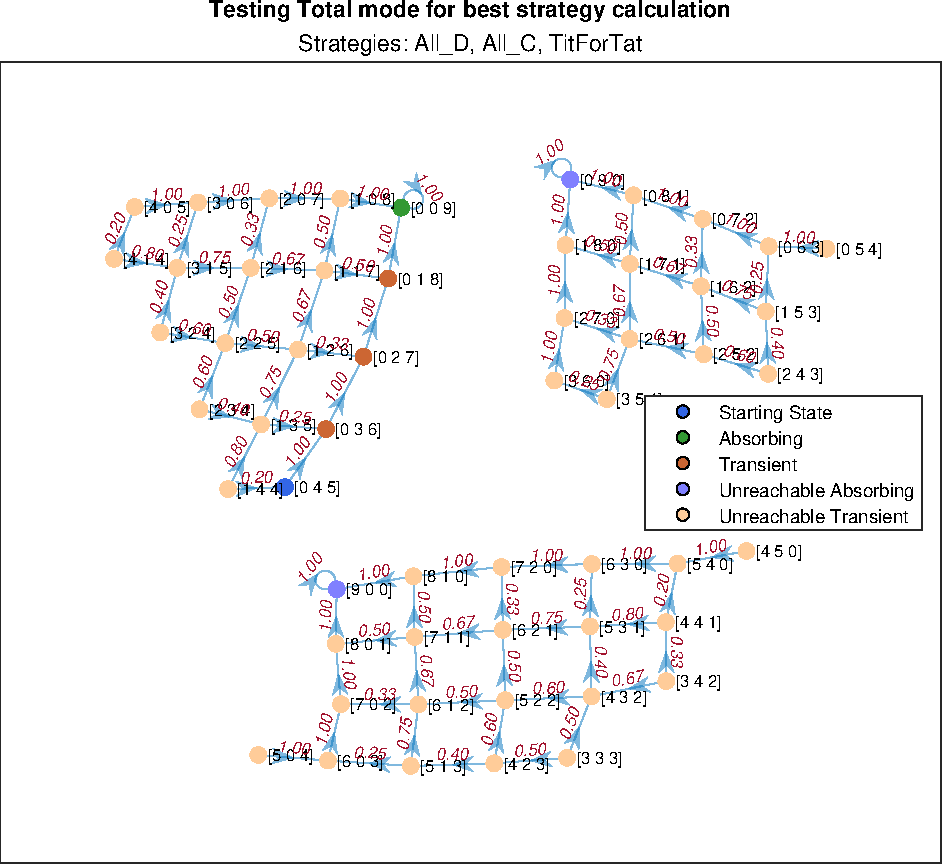
\includegraphics[width=0.95\textwidth]{Testing Total mode for best strategy calculation}
	      \caption{Testing ``Total'' mode for best strategy calculation with $POP0=\begin{bmatrix}1&4&5\end{bmatrix}$}
	      \label{fig:TourTheImiTotal}
	\end{figure}
